\section{Corpus}
\label{sec:corpus}

\subsection{Constitution, sources du corpus}
\label{subsec:corpus_constitution}

\subsection{Répartition chronologique du corpus}
\label{subsec:corpus_chrono}

\begin{figure}[]
    \centering
    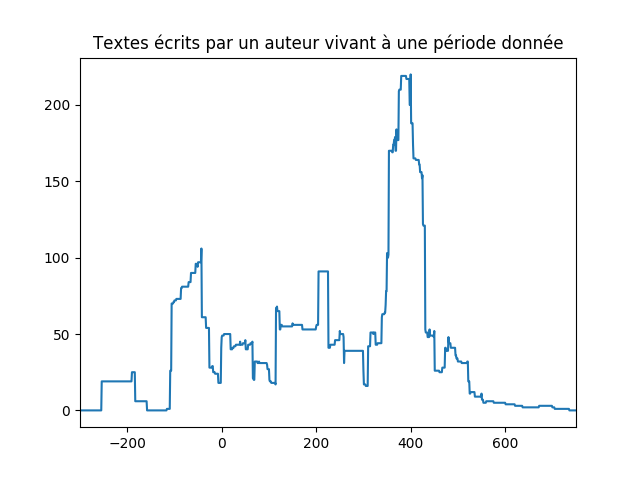
\includegraphics[width=10cm]{results/analysis/corpus_analysis/texts_per_year.png}
    \caption{Répartition des textes en fonction de l'année de naissance et de mort de l'auteur}
    \label{texts_per_year}
\end{figure}

\begin{figure}[]
    \centering
    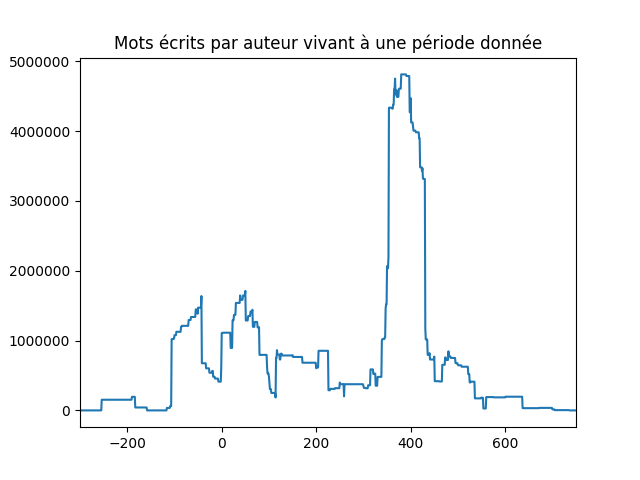
\includegraphics[width=10cm]{results/analysis/corpus_analysis/tokens_per_year.png}
    \caption{Répartition des mots en fonction de l'année de naissance et de mort de l'auteur}
    \label{tokens_per_year}
\end{figure}

\begin{figure}[]
    \centering
    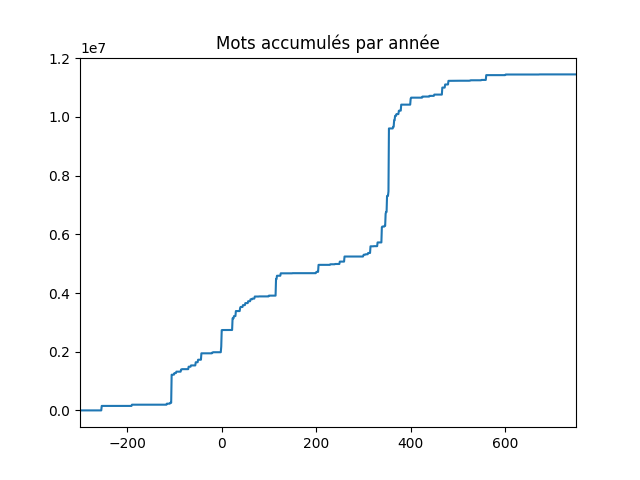
\includegraphics[width=10cm]{results/analysis/corpus_analysis/accumulated_tokens.png}
    \caption{Nombre de mots accumulés au fil des années}
    \label{accumulated_tokens_per_year}
\end{figure}


\paragraph{Méthodes de datation}

\subsection{Découpage du corpus}
\label{subsec:corpus_decoupage}

\begin{figure}[]
    \centering
    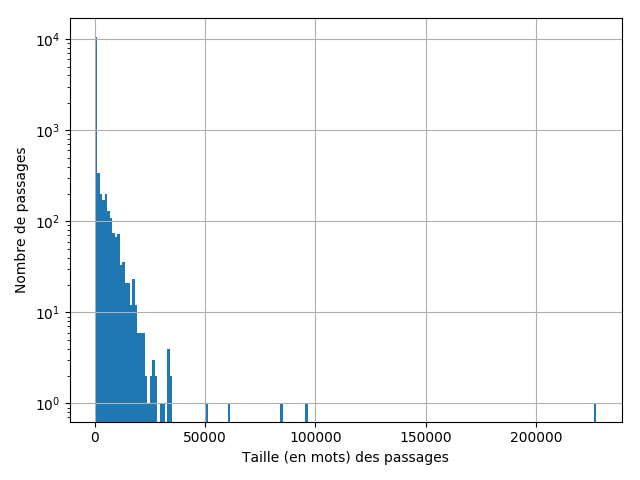
\includegraphics[width=10cm]{results/analysis/corpus_analysis/passage_size_distribution.png}
    \caption{Répartition des tailles (en mots) d'extraits}
    \label{passage_size_distribution}
\end{figure}

\subsection{Statistiques lexicales du corpus}
\label{subsec:corpus_lexical_stats}

\subsection{Risques de répétition : analyse des doublons}
\label{subsec:corpus_repetition}

Basé sur l'étude de l'impact des duplications de texte en topic modeling \footcite{schofield2017quantifying}, nous proposons ici une expérience
quant à la nécessité pour le corpus d'être soigné.